\documentclass[a4paper, titlepage]{article}
\usepackage[a4paper,top=2.5cm,bottom=2.5cm,left=3cm,right=3cm]{geometry}
\usepackage[T1]{fontenc}
\usepackage[utf8]{inputenc}
\usepackage[italian]{babel}
\usepackage{float}
\usepackage{graphicx}
\usepackage{rotating}
\usepackage{siunitx}  
\graphicspath{ {images/} }
\usepackage[rightcaption]{sidecap}
\usepackage[dvipsnames]{xcolor}
\usepackage{subfigure}
\usepackage{hyperref}
\usepackage{amsmath}


\begin{document}
\begin{titlepage}
	\centering
	{\scshape\Large Relazione di laboratorio\par}
	\vspace{0.7 cm}
	\hrule
	\vspace{1.2 cm}
	\begin{figure}[!h]
	    \centering
	    
\includegraphics[width=0.30\textwidth]{Politecnico_di_Torino_-_Logo}
        %\includegraphics[width = 0.50\textwidth]{ITA-template-mesap-01}
	\end{figure}
	
		\vspace{1 cm}
	{\huge\bfseries Progettazione di un'interfaccia  UART per comunicazione  RS-232\par}
	
	\vspace{2 cm}
	Corso di Laurea Magistrale in Ingegneria Elettronica\par
	\null
	\vfill
	{\raggedright\small Studenti\\\large  Amato Giovanni Luca Matr.267511	\\Cerbai Matilde Matr.274908 \\Chisciotti Laura Matr.274728\\Goti Gianluca Matr.269825\par}
	\vspace{0.2 cm}

	\vfill
	{\large A.A. 2019/20}
\end{titlepage}
\newpage
\tableofcontents
\newpage
\section{Il protocollo RS-232}
\subsection{Caratteristiche generali}
L'RS-232 è uno standard che permette lo scambio di informazioni a bassa velocità tra dispositivi digitali.
Tale protocollo presenta tre caratteristiche principali:
\begin{itemize}
\item Seriale; 
\item Full-duplex;
\item Asincrono;
\end{itemize}
Questo significa che è possibile trasmettere e ricevere contemporaneamente solo un bit alla volta  e non viene scambiato alcun tipo di clock.\\
Nella sua forma più semplice, tale protocollo ha un supporto fisico costituito da due fili,  "Tx" e  "Rx", anche se nella realtà è più complesso, infatti presenta molte più connessioni dato che è stato progettato per comunicazioni a lunga distanza, dell'ordine di una decina di metri.\\
Per quanto concerne i livelli logici, non vengono usati dei valori di tensione comuni, motivo per cui tale protocollo è molto robusto, infatti si può avere fino a 9V di margine di rumore.\\
In uscita è presente:
\begin{itemize}
\item +12 V = $0$ Logico "V$_{OL}$"
\item -12 V = $1$ Logico "V$_{OH}$"
\end{itemize}
In ingresso è possibile trovare fino a:
\begin{itemize}
\item +3 V = "V$_{IL}$"
\item -3 V = "V$_{IH}$"
\end{itemize}
Naturalmente queste non sono tensioni logiche normali, esistono dei circuiti (MAX232) che trasformano tali livelli logici in TTL o CMOS compatibili e viceversa.
\subsection{Descrizione del segnale}
Lo standard trasmette un bit alla volta, ogni word da 8 bit è incapsulata (framing) con un bit di "START" ( 0 logico) e un bit di "STOP" (1 logico), il livello "neutro" è l'"IDLE" ( 1 logico). In generale le combinazioni possono essere molteplici, deve essere presente un accordo esplicito sulla lunghezza della word trasmessa, il bit di stop può durare per uno o più tempi di bit,  inoltre ci può essere parità o meno.\\
Nel caso sotto esame il protocollo prevedeva:
\begin{itemize}
\item 8 bit (word)
\item No parity
\item 1 bit di STOP
\end{itemize}
Quando il sistema è in quiete si trova nello stato di "IDLE", che equivale all' "1" logico. Quando l'utente vuole iniziare una trasmissione ci deve essere sempre una transizione, infatti da "IDLE" si passa a "START" ottenendo così una transizione dall' "1" logico allo "0" logico. Il bit di "STOP" è importante in quanto se l'utente vuole effettuare una trasmissione continua, la transizione "1" logico e "0" logico è sempre garantita, poichè lo "STOP" riporta a livello alto la linea garantendo così la corretta transizione.\\
Il timing diagram di una generica trasmissione RS-232 si presenta come in Figura \ref{fig:timing_RS}
\pagebreak
\begin{figure}[h]
\centering
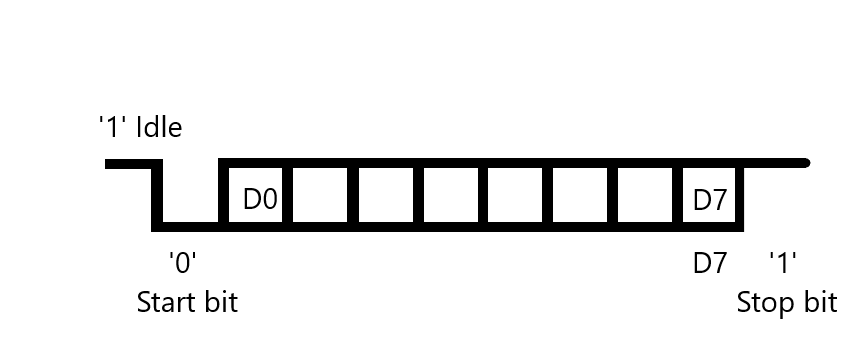
\includegraphics[scale=0.5]{RS232}
\caption{Timing diagram di una generica trasmissione RS-232}
\label{fig:timing_RS}
\end{figure}\\
Come è possibile notare nella figura e come già detto in precedenza, il sistema passa da uno stato di quiete, ovvero "IDLE", al bit di "START", eseguendo così la transizione che farà capire al ricevitore che è stata iniziata una nuova trasmissione. Infine il sistema passa in "STOP" e dopodichè ( se non vi è una nuova trasmissione) ritorna in "IDLE".

\section{Struttura generale della UART}
In Figura \ref{fig:UART} è stata riportata la struttura della UART progettata.\\L'obiettivo è stato quello di realizzare un'unità di ricezione e di trasmissione seriale di dati secondo il protocollo RS-232 precedentemente introdotto.\\Il trasmettitore e il ricevitore sono stati realizzati indipendentemente, ma in modo tale da riuscire ad interfacciarsi nel rispetto delle specifiche a disposizione.
\begin{figure}[h]
    \centering
    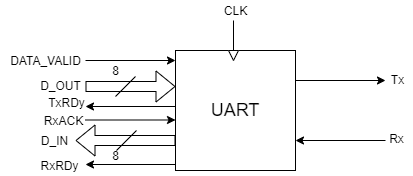
\includegraphics[scale=0.8]{UART.png} 
    \caption{UART}
    \label{fig:UART}
\end{figure}
\section{Trasmettitore}
\subsection{Struttura e caratteristiche principali}
In riferimento alla Figura \ref{fig:UART}, sono osservabili i principali segnali che arrivano e che partono dalla UART e che interessano il trasmettitore.
\begin{itemize}
\item \textbf{D\_OUT}: bus da 8 bit, che carica in modo parallelo il dato che deve essere trasmesso;
\item \textbf{Data\textunderscore Valid}: segnale in ingresso, che dice al trasmettitore quando campionare il dato da trasmettere;
\item \textbf{TX\_RDY}: segnale di stato del trasmettitore, comunica all'esterno se il sistema è in trasmissione (busy) o meno;
\item \textbf{TX}: uscita seriale del trasmettitore.
\end{itemize}
Quando il trasmettitore non lavora, il TX\_RDY è tenuto alto, mentre quando è in trasmissione tale segnale è basso (busy).\\Il funzionamento di tale trasmettitore è abbastanza semplice:
\begin{itemize}
\item L'utilizzatore esterno, per esempio un $\mu$C, manda la word che vuole trasmettere al bus D\_OUT;
\item Dopo aver mandato il dato da trasmettere (e mantenendolo per il tempo necessario)  asserisce il Data\_Valid, in questo modo il trasmettitore campiona i dati che dovrà trasmettere;
\item Il trasmettitore acquisisce i dati e li trasmette seguendo la logica del protocollo e pone al livello logico basso la linea TX\_RDY;
\item Dopo che la trasmissione è finita, il TX\_RDY è posto a livello logico alto e il sistema è pronto per una nuova trasmissione.
\end{itemize}
Il sistema lavora con un clock da 25 MHz, la trasmissione seriale è a 9600 baud e ciò significa che il tempo di bit è circa 104 $\mu$s Perciò, una trasmissione completa, che comprende quindi sia il bit di "START" e di "STOP", ha una durata di circa 1040 $\mu$s.
\subsubsection{Data Path}
Il datapath del trasmettitore è mostrato in Figura \ref{fig:dpath_TX}.
\begin{figure}[h]
\centering
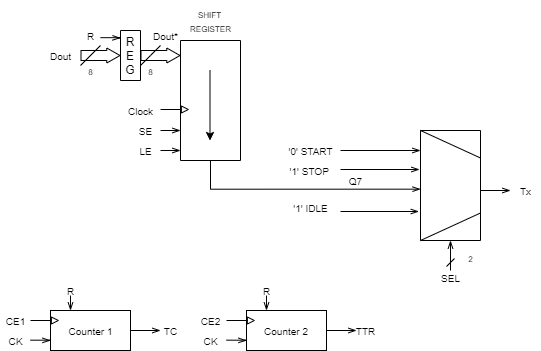
\includegraphics[scale=0.8]{datapath_tx.png}
\caption{Datapath del trasmettitore}
\label{fig:dpath_TX}
\end{figure}
\\Lo shift register è il cuore di questo sistema, infatti è tale componente che esegue la "serializzazione" del dato, in particolare questo ha un caricamento di tipo parallelo, una porta che abilita lo shift "SE" (shift enable) e una porta che abilita il load "LE" (load enable).\\Idealmente appena il sistema avverte il Data\_Valid, lo shift register dovrebbe caricare i dati all'interno, questo però comporterebbe la creazione di una macchina di Mealy, in quanto un segnale esterno provoca un'immediata reazione nella macchina.\\Ovviamente si vuole evitare in ogni modo tale situazione, infatti la soluzione adottata è la macchina di Moore, per questo il sistema risponde al Data Valid con un comando di "load" dello Shift register al colpo di clock successivo. Risulta quindi immediatamente evidente la necessità di un registro che permetta di ritardare del tempo necessario, in questo caso un colpo di clock, per dare la possibilità al sistema di rispondere correttamente e quindi di campionare il dato, caricandolo così all'interno dello shift register. La temporizzazione della trasmissione è accertata da due contatori, il "Counter 1", che assicura la corretta temporizzazione tra la trasmissione di un bit e l'altro, ed il "Counter 2", che conta il numero di bit trasmessi durante la comunicazione, decretandone in seguito la fine. Entrambi i contatori hanno un terminal count che viene mandato alla Control Unit (CU), la quale risponde al colpo di clock successivo col comando corretto (può per esempio abilitare lo shift dello shift register oppure girare il mux).
\subsection{Control Unit}
La Control Unit (CU) utilizzata per questo progetto è costituita da una parte sequenziale che fa progredire gli stati, occupandosi quindi anche di eventuali salti e una parte puramente combinatoria che manda i comandi al data path. In Figura \ref{fig:fsm} è presente uno schema di principio della CU utilizzata.
\begin{figure}[h]
\centering
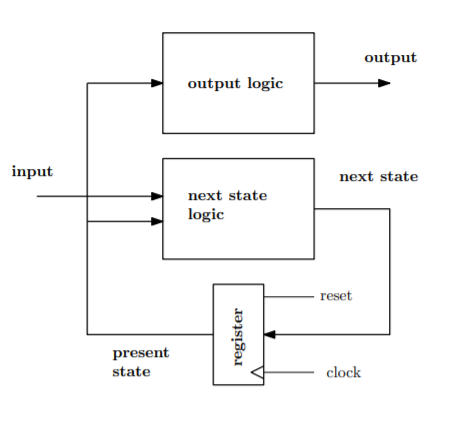
\includegraphics[scale=0.6]{fsm_2processi}
\caption{FSM a due processi}
\label{fig:fsm}
\end{figure}\\
Come si può notare dalla figura, gli input entrano nella "next state logic", ma sono filtrati da un registro, che permette di svincolarsi dall'esterno, evitando di creare una macchina di Mealy. Nel progetto, ogni volta che un segnale arriva dal data path ed entra nella CU, provoca una risposta di questa con un adeguato comando solamente al colpo di clock successivo.
\newpage
\subsection{Diagramma di stato}
In Figura \ref{fig:palloTX} è riportato il diagramma di stato del trasmettitore, dove per ragioni di chiarezza e pulizia dello schema non sono state incluse tutte le connessioni che portano allo stato di "RESET", attivate con la condizione "RST=1".\\
\begin{figure}[h]
    \centering
    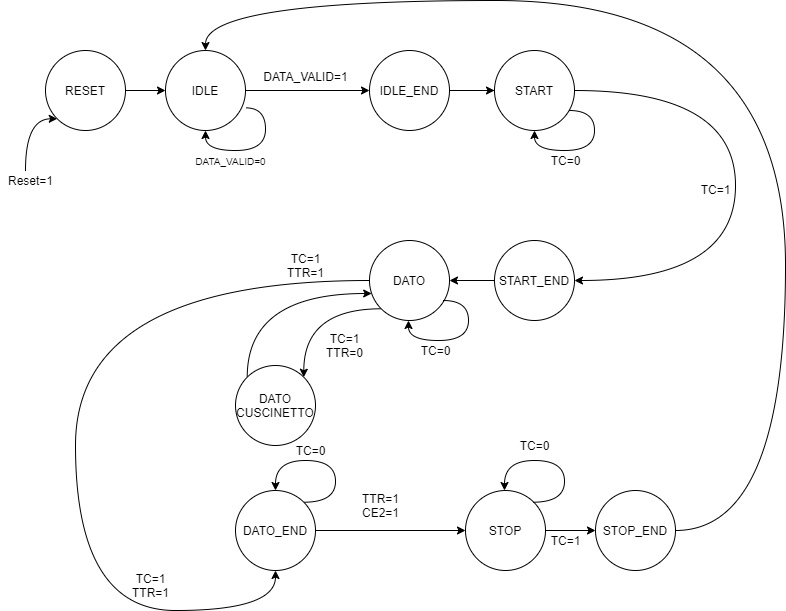
\includegraphics[scale=0.6]{PalleogrammaTx_V2 (2).png}
    \caption{Diagramma di stato del trasmettitore}
    \label{fig:palloTX}
\end{figure}\\
Come è possibile notare dal diagramma, il sistema rimane in stato di "IDLE" finché non riceve il segnale "DATA\textunderscore VALID=1", in seguito, dopo essere transitati dallo stato "IDLE \textunderscore END" il sistema approda in "START" dove, con la progressione allo stato successivo, verranno dati i comandi per inviare il bit di start. In tale stato vi può essere una progressione solamente se il segnale "TC=1", cioè il terminal count del contatore che garantisce il tempo di bit. Se tale condizione non è verificata il sistema rimane nello stato attuale. Nello stato "DATO" il sistema resta in attesa della condizione "TC=1", che permette di saltare in "DATO\_CUSCINETTO e di mandare quindi in uscita i comandi necessari allo shift register per far uscire i dati in sequenza (in questo caso è stato creato un loop per inviare tutti gli 8 bit della trasmissione) . Dopodiché il sistema  torna nello stato "DATO", dove vengono abbassati tutti i comandi relativi all'invio dei dati. Inoltre il dispositivo contiene un contatore, che conta i bit di dato trasmessi ed ilcui terminal count ("TTR") viene alzato quando conta 7. Tale segnale è stato sfruttato per generare una condizione di salto insieme alla condizione "TC=1", quindi, quando questa è verificata, si salta nello stato che manda in uscita l'ultimo bit e che permette di preparare il sistema ad inviare il bit di stop, una volta giunti nello stato "STOP \textunderscore END", la CU gira il mux per inviare il bit di "IDLE" e in seguito il sistema torna in quiete nello stato di "IDLE", in attesa di una nuova trasmissione e quindi di un nuovo "DATA \textunderscore VALID".
\subsection{Timing Diagram}%versione MATI con integrazioni DP
In Figura \ref{TX Timing} è riportato il timing del trasmettitore, di cui sono state analizzate alcune sue parti in riferimento ai segnali interessati:
\begin{itemize}
\item 	\textbf{Clk}: clock a 25 MHz;
\item 	\textbf{Dout}: word da trasmettere;
\item 	\textbf{Data valid}: segnale che identifica quando il dato può essere campionato;
\item 	\textbf{SE}: shift enable dello shift register;
\item 	\textbf{TxRDy}: segnale che identifica quando la UART può trasmettere;
\item 	\textbf{LE}: load enable dello shift register;
\item 	\textbf{Dout*}: Dout ritardato di un colpo di clock;
\item 	\textbf{SEL}: select del mux;
\item 	\textbf{CE1}: counter enable del COUNTER 1, che fornisce il tempo di bit;
\item 	\textbf{TC}: terminal count del contatore 1;
\item 	\textbf{Tx}: uscita seriale del trasmettitore;
\item 	\textbf{CE2}: counter enable del COUNTER 2;
\item 	\textbf{TTR}: terminal trasmission del contatore 2;
\item \textbf{Reset}: reset del sistema;
\end{itemize}
Il flow del timing diagram è il seguente:
\begin{enumerate}
    \item Dout è il dato da trasmettere, l'utilizzatore, per esempio un PC o un $\mu$C, pone la word sul bus;
    \item l'utilizzatore invia il Data\_Valid quando il dato da trasmettere è stabile. Tale segnale comunica alla UART che può campionare il dato, caricandolo così istantaneamente i dati nello shift register. Questa situazione, però, ci riporterebbe ad una macchina di Mealy, caso da evitare;
    \item a tal proposito, il segnale da trasmettere è ritardato di un colpo di clock ed è indidato con  Dout*. Questo permette anche di svincolarsi dal mondo esterno;
    \item il load enable (LE), per creare una macchina di Moore, é attivato al colpo di clock successivo al Data\_Valid, permettendo così di caricare i dati all'interno dello shift register;
    \item nel momento in cui il dato viene campionato, lo shift enable dello shift register (SR) è disabilitato, evitando così di shiftare il dato appena caricato;
    \item TxRDy passa quindi da livello alto a basso, comunicando che è in corso una trasmissione (stato "Busy");
    \item nello stesso istante, il contatore 1 è abilitato per contare il tempo necessario per trasmettere un bit. Il segnale terminal count (TC) viene attivato tutte le volte che sarà passato tale lasso di tempo (1 bit trasmesso);
    \item l'uscita dello shift register porta il dato shiftato in ingresso al multiplex;
    \item il comando SEL permette di girare il mux, secondo codifica, per trasmettere IDLE (00);
    \item Tx, che rappresenta l'uscita del mux, passa quindi dallo stato IDLE allo START al colpo di clock successivo alla ricezione del TC da parte della control unit;
    \item Dopo la trasmissione del bit di START il sistema è in quiete finché il TC non diventa alto. Al colpo di clock successivo la control unit invia i comandi necessari per lo shift del dato in uscita (SE) e l'abilitazione del contatore 2 (CE2), che conta il numero di bit della word che sono stati trasmessi;
    \item il segnale Terminal trasmission (TTR) indica la fine della trasmissione della word e sarà attivo dal momento in cui viene contato il passaggio dell'ottavo bit a quando il mux non viene girato per trasmettere STOP;
    \item Per completezza è stata anche inserita la routine di reset, la quale disabilita i counter enable, il load enable e lo shift enable dello shift register, pone il TX\_RDY in modalità "Busy" e pone il mux in posizione "00" così da trasmettere lo stato di "IDLE" in uscita.
\end{enumerate}

\subsection{Simulazione su Modelsim}
Per valutare in prima fase il corretto funzionamento del trasmettitore, si è sfruttato il software Modelsim per effettuare svariate simulazioni con word di 8 bit scelte arbitrariamente, si riporta di seguito, in Figura \ref{fig:testTx} , a titolo di esempio una simulazione effettuata. 
\begin{figure}[h]
    \centering
    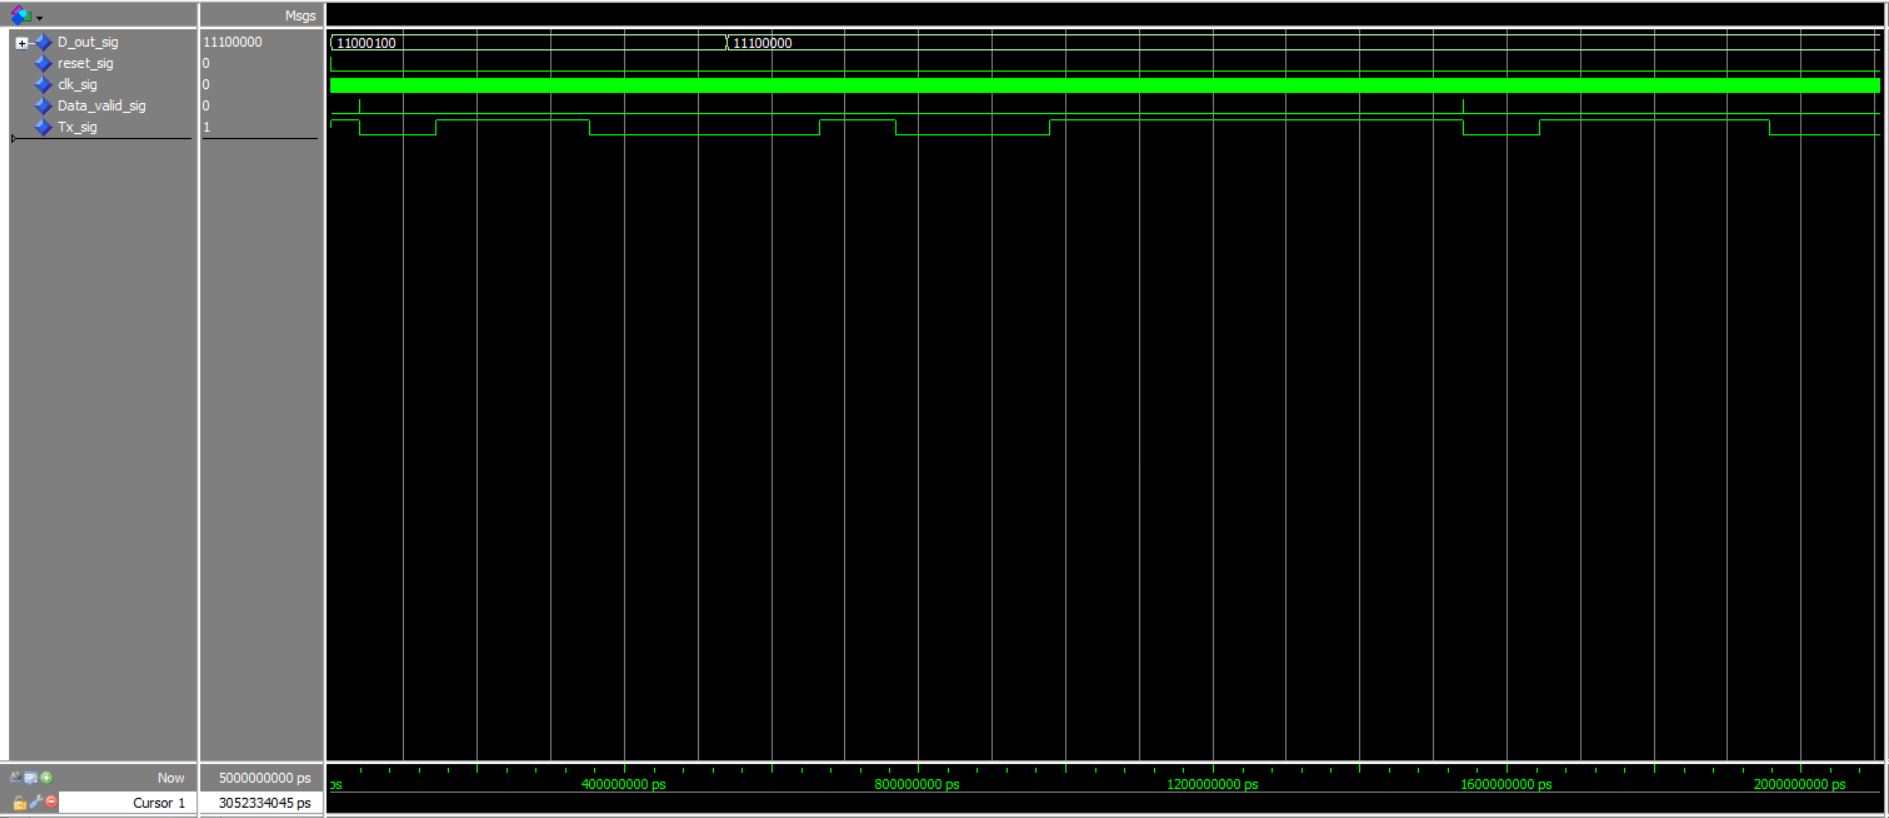
\includegraphics[scale=0.4]{test_TX_modelsim.PNG}
    \caption{Simulazione di una trasmissione}
    \label{fig:testTx}
\end{figure}\\
\noindent Dalla simulazione è possibile osservare che il sistema inizialmente si trova in "IDLE" (linea Tx alta), dopo aver applicato il "DATA \textunderscore VALID" il sistema invia il bit di start (linea bassa) e poi inizia la trasmissione partendo dall'LSB della word. Alla fine della trasmissione il sistema manda il bit di stop (linea alta) e torna in "IDLE", in attesa di una nuova word da trasmettere, ciò è da poter notare dalla simulazione, in quanto la linea TX rimane alta in attesa di un nuovo "DATA \textunderscore VALID".
\newpage
\subsection{Test su board DE1}
In seguito sono stati effettuati dei test sulla Board Altera DE1 presente in laboratorio, si è reso quindi necessario la progettazione di un testbench "hardware" per verificare il funzionamento del trasmettitore attraverso l'oscilloscopio. Lo schema del testbench progettato è mostrato in Figura \ref{fig:my_testTX}.
\begin{figure}[h]
    \centering
    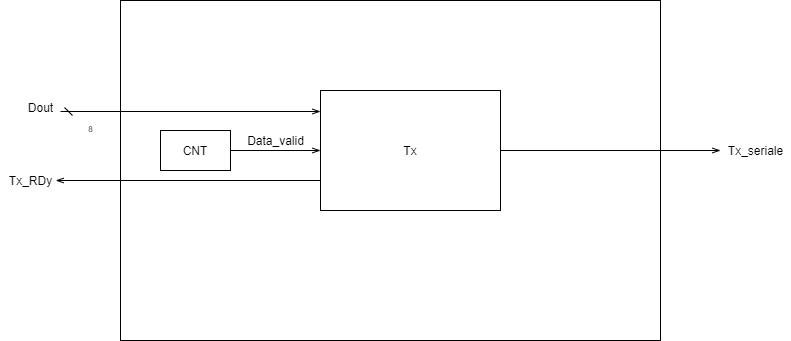
\includegraphics[scale=0.5]{test_tx.png}
    \caption{Schema test HW per il trasmettitore}
    \label{fig:my_testTX}
\end{figure}\\
\noindent Per valutare il corretto funzionamento del trasmettitore, è stata sviluppata una top-level entity contenente il trasmettitore e un contatore il cui terminal count è stato collegato al Data Valid. Il valore del contatore è stato settato in modo da inviare un DATA \_VALID ogni 1,25 s così da permettere la visualizzazione della trasmissione sull'oscilloscopio. Il bus Dout è stato collegato agli switch della board DE1, così da variare il dato trasmesso ed il risultato è stato verificato attraverso l'oscilloscopio. Di seguito in Figura \ref{fig:test_osc} è riportato, a titolo di esempio, un test effettuato in laboratorio dove è stata trasmessa la word "01100100", in cui il primo bit a sinistra rappresenta l'LSB.\\Come impostazioni sono stati posti 100$\mu$s/DIV, in modo tale da poter vedere circa un bit per divisione, dato che ciascun bit ha la durata di 104$\mu$s. Inoltre sull'oscilloscopio è osservabile a sinistra, prima dell'LSB, il bit di IDLE (1) ed il bit di START(0), ed a destra, successivo all'MSB, il bit di STOP (1). Successivo al bit di STOP, è possibile osservare che ci sono ancora qualche altro $\mu$s a livello logico alto, questi rappresentano una frazione dell'IDLE, facente parte della seconda word trasmessa.
\begin{figure}[h]
    \centering
   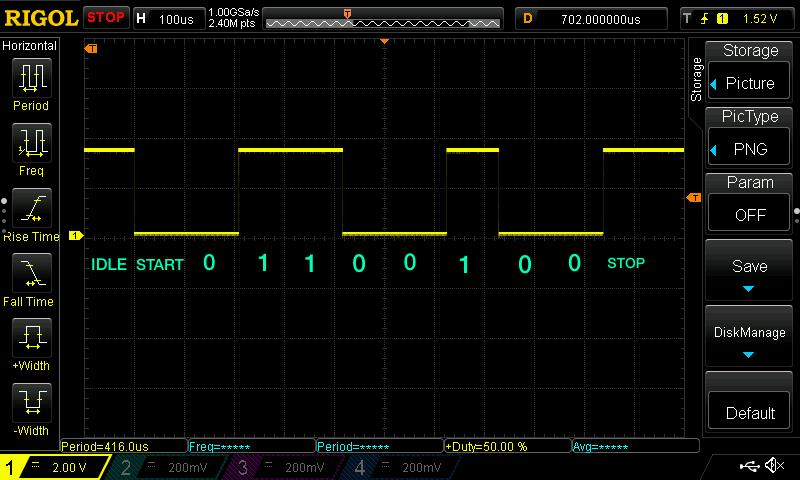
\includegraphics[scale=0.5]{trasmissione su oscilloscopio.jpeg}
    \caption{Test su oscilloscopio}
    \label{fig:test_osc}
\end{figure}
\section{Ricevitore}
In tale sezione è stato analizzato il blocco di ricezione della UART realizzata secondo le specifiche di progetto, il quale, per attuare al meglio le metodologie apprese, é stato idealmente considerato indipendente dal trasmettitore, assumendo quindi un segnale di clock differente.
\newline
%\\Tutto il progetto è stato realizzato considerando che il ricevitore risulta essere indipendente dal trasmettitore, non avendo lo stesso clock.
Come è stato precedentemente detto, il Tx lavora a 9600 baud, ma non disponendo di un riferimento temporale è stato considerato che il bit di START potesse arrivare in qualsiasi momento, com'é ragionevole aspettarsi in una comunicazione reale. Per gestire tale situazione è stato deciso di sovracampionare ciascun bit di un fattore 8, andando ad aumentare il baud rate (9600x8), in modo tale da riuscire a capire quando effettivamente il bit ricevuto fosse quello di START e dove avvenisse la transizione da IDLE, cioè livello logico alto, a START, corrispondente a livello logico basso.\\Come verifica della reale avvenuta transizione, è stato posto di rilevare questa solo nel momento in cui sono presenti nel primo shift register quattro 1, riferiti all'IDLE, e quattro 0, relativi allo START. Tale condizione è stata verificata tramite l'utilizzo di una semplice porta AND, che pone l'uscita a 1 se e solo se è verificata la condizione precedentemente esposta.\\ Finché tale condizione è vera l'AND mantiene alto il segnale di "START TRANSITION", che indica la transizione da livello logico alto a basso. Questo si abbasserà successivamente con l'arrivo del quinto bit di START.\\Per esplicitare meglio il concetto è stato riportato il disegno in Figura \ref{fig:my_label}.
\begin{figure}[h]
    \centering
    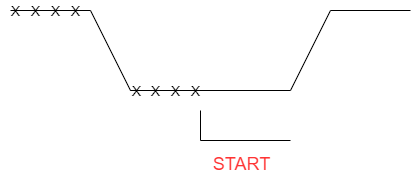
\includegraphics[scale=0.6]{Rx.png}    \caption{START Transition}
    \label{fig:my_label}
\end{figure}\\
\subsection{Struttura e caratteristiche principali}
In riferimento alla Figura \ref{fig:UART}, sono stati considerati i principali segnali che interessano il ricevitore:
\begin{itemize}
    \item \textbf{D \_IN}: bus da 8 bit, che presenta in parallelo il dato ricevuto in modo seriale;
    \item \textbf{RX}: segnale di ingresso seriale del ricevitore;
    \item \textbf{RX\_RDy}: tale segnale è messo alto o basso dal ricevitore stesso, se è alto vuol dire che il sistema è in ricezione e non può ricevere una nuova word;
    \item \textbf{RX\_ACK}: se asserito indica che la word ricevuta è stata acquisita dal sistema utilizzatore;
\end{itemize}
\newpage
\subsection{Datapath} 
Nella figura sottostante è stato riportato il datapath del ricevitore:
\begin{figure}[h]
    \centering
    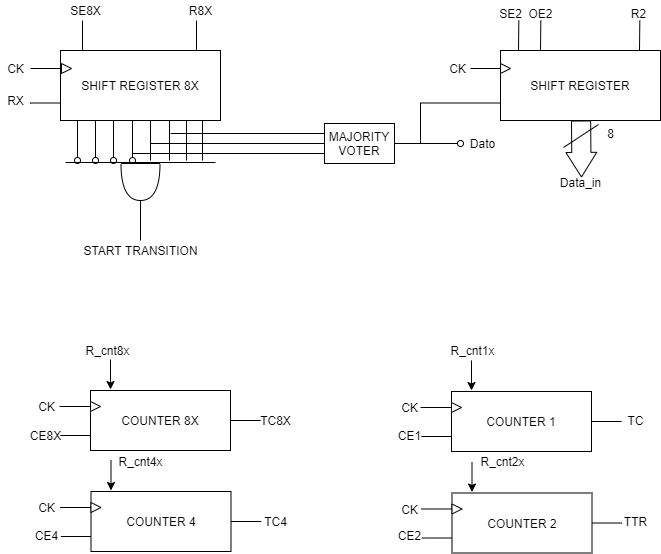
\includegraphics[scale=0.4]{DatapathRx (3).png}
    \caption{Datapath ricevitore}
    \label{fig:dp_rx}
\end{figure}
\\\\
\\\\ Data la word di 8 bit di cui è composto ogni dato, è stato considerato uno shift register 8x, che risulta essere sempre attivo in modo tale da shiftare sempre i bit e effettuare il sovracampionamento. Il majority voter (MV): permette di prendere il valore al centro del bit. Tale blocco considera più campioni adiacenti, nel caso specifico 3 bit per eliminare il minore e prendere il valore che compare più volte nei 3 bit scelti, cioè o 0 o 1. E' stato deciso di prendere i bit 2,3 e 4 dello shift register in quanto, dopo altri quattro shift a partire dall'individuazione dell'inizio di una nuova trasmissione, lo shift register risulta essere "riempito" da tutti gli 8 campioni di un generico bit della word e quelle specifiche posizioni risultano essere in posizione centrale (in termini temporali) al bit. %(HO CONTROLLATO E VANNO BENE).
\\
Come già spiegato, l'individuazione dello start transition non serve solo a capire quando avviene una nuova trasmissione, ma serve anche a posizionarsi al centro del bit. Infatti dopo altri quattro shift dello shift register, che opera il sovracampionamento, questo sarà riempito da tutti gli 8 campioni del bit di start, questo rende possibile l'individuazione del centro del bit, posizionando in modo opportuno il majority voter. Trascorso un tempo di bit, cioè 8 campionamenti a una velocità 8x, all'interno del majority voter "entra" il nuovo centro del bit della word.\\
L'uscita del MV, entrerà nel secondo shift register, che viene attivato tramite il comando OE2 solo ogni 8 shift del primo Shift Register, una volta che viene riempito di tutti gli 8 bit della word, il comando di output enable viene abilitato e la word è mandata in uscita sul bus DATA\_in.\\ Si hanno quattro contatori che garantiscono l'adeguata temporizzazione di segnali che interessano la parte di ricezione:
\begin{itemize}
    \item counter8x: conta 324 colpi di clock ed assicura il sovracampionamento 8X,
    \item counter 1: conta 2603 colpi di clock, assicurando il tempo di bit (9600 baud),
    \item counter 2: conta i bit della word ricevuti,
    \item counter 4: conta 4 shift, permettendo così l'individuazione del centro del bit.
\end{itemize}
%Fatto check
\newpage
\subsection{Timing Diagram}
Il timing relativo all'operazione di ricezione è stato riportato in Figura \ref{RX Timing}, la quale è situata alla fine di tale relazione.\\
I segnali interessati nell’operazione di ricezione sono i  seguenti:
\begin{itemize}
\item 	\textbf{Clk}: clock a 25 MHz;
\item 	\textbf{D\_IN}: dato trasmesso. E' l'uscita del secondo shift register;
\item \textbf{Reset}: quando RST=1 il reset riporta il sistema di elaborazione allo stato iniziale;
\item 	\textbf{Rx\_RDY}: segnale con cui la UART comunica al $\mu$processore che il secondo shift register è pronto per mandare in uscita D\_IN;
\item 	\textbf{Ack}: indica 'acknoledge' e si attiva quando il $\mu$processore ha ricevuto tutto il dato. E' il $\mu$processore stesso che manda alla UART tale segnale;
\item 	\textbf{Rx}: bit trasmessi;
\item 	\textbf{TC8X}: rappresenta il terminal count (uscita) del contatore, che conta 325 colpi di clock;
\item 	\textbf{SE8x}: è lo shift enable del contatore COUNTER 8x 
\item 	\textbf{STR}: indica la start trasmission e si ha quando è stata identificata una transizione di START;
\item 	\textbf{CE8x}: è il counter enable del contatore 8x;
\item 	\textbf{TC4x}: è il terminal count del contatore 4x, che conta 4 shift;
\item 	\textbf{CE4}: counter enable del contatore 4x
\item 	\textbf{CE1}: counter enable del COUNTER 1, che conta 2603 colpi di clock;
\item 	\textbf{TC}: terminal counter del COUNTER 1, viene inviato quando termina di contare;
\item 	\textbf{SE2}: shift enable del secondo shift register;
\item 	\textbf{CE2}: counter enable del COUNTER 2, che conta i bit ricevuti;
\item 	\textbf{TTR}: terminal trasmission, è l'uscita del COUNTER 2, che viene inviata quando termina di contare;
\item 	\textbf{OE2}: output enable del secondo shift register;
\end{itemize}
Di seguito sono riportati alcuni chiarimenti per comprendere più facilmente il timing:
\begin{enumerate}
    \item dato che la trasmissione è continua, Rx parte come attivo alto ("IDLE");
    \item l'asserimento di TC8X permette l'attivazione di SE8X. Questi due sono asseriti per un solo colpo di clock. Ciò consente di sovracampionare il dato in ricezione ad una velocità 8x. Tale processo è continuo ed è necessario in quanto la ricezione di una nuova word non può essere predetta, quindi non è possibile sapere temporalmente quando lo START, mandato dal trasmettitore, sarà ricevuto;
    \item quando nel primo shift register sono presenti quattro 0  (dello start) e quattro 1 (dell'idle), c'è la sicurezza di ricevere una transizione di inizio trasmissione ("START"), quindi a livello di timing avviene l'asserimento del segnale STR. Ciò viene verificato in concomitanza con l'abbassarsi dello shift enable (SE8X) del quarto zero dello start.\\Il segnale STR, dato che è prodotto da una porta AND, rimane alto finché lo shift register non fa scorrere un nuovo dato al suo interno;
   % \item Dopo l'asserimento del segnale STR, il segnale Rx viene abbassato e avviene uno shiftaggio di zeri all'interno del primo shift register;
    \item CE4X viene asserito un colpo di clock dopo che STR è stato alzato.\\ CE4X abilita il COUNTER 4, che deve contare 4 shift (del sovracampionatore) in modo tale da far entrare tutti gli 8 bit di start e quindi di centrare questo rispetto al VOTER;
    \item Durante il processo di ricerca della transizione dello start, SE2 non è asserito, quindi il secondo shift register è disabilitato in quanto è stato scelto di estrapolare la word dal frame ricevuto;
    \item TC4X indica il termine dello shift degli ultimi 4 zeri dello start e viene asserito dal contatore in concomitanza del TC8X dell'ultimo bit di start (questo perchè i conteggi stanno in un rapporto 1:4), per essere poi abbassato al colpo di clock successivo;
    \item in contemporanea all'asserimento dello shift enable riferito all'ultimo bit dello start, viene disabilitato il CE4X precedentemente attivato e viene asserito il CE1, il quale fa partire il conteggio di 2603 colpi di clock, che assicura il tempo di bit;
    \item Dopo lo shift dell'ultimo bit di start, iniziano ad essere ricevuti i bit del dato trasmesso. Per tali bit va fatto riferimento ai segnali TC e SE2, che indicano quando entrano i bit del dato trasmesso nel secondo shift register.\\ In questo momento ci sono contemporaneamente uno shiftaggio nel primo shift register ed uno nel secondo shift register, dato che il COUNTER 1 è abilitato a contare dall'asserimento del CE1 e questo porta ad introdurre all’interno del secondo shift register i singoli bit valutati dal Majority Voter dopo il sovraccampionamento;
    \item Una volta che il secondo shift register è riempito dagli 8 bit della word trasmessa, il CE2, che era stato alzato in concomitanza dello shift enable (SE2) del primo dato tramesso, va basso, poichè sono stati ricevuti tutti i bit necessari;
    \item Contemporaneamente all'abbassarsi del CE2, il segnale TTR va alto, per poi abbassarsi al colpo di clock successivo. Questo indica che la trasmissione è terminata e che sono stati ricevuti tutti i bit della word (8 bit);
    \item La word viene mandata in uscita sul bus e l'Output enable del secondo shift register è asserito, il sistema inoltre pone la linea RX\_Rdy a livello logico alto, indicando così che un dato ricevuto è disponibile;
    \item Una volta che il sistema utilizzatore ha campionato il dato, fornisce il segnale Ack per un unico colpo di clock, al colpo successivo l' RX\_Rdy e OE2 sono disattivati ed il sistema rimane in attesa di una nuova ricezione;
    \item Se viene mandato il Reset alto, il cui asserimento dura un unico colpo di clock,tutte le impostazioni vengono resettate, riportando il sistema alle condizioni iniziali. Tutti i segnali di enable dei contatori e degli shift register sono disabilitati, oltre al reset dei componenti stessi, Inoltre è disattivato anche il counter enable, che permette di sovracampionare. 
    \end{enumerate}.
\newpage
\subsection{Diagramma di stato}
Nella figura sotto è riportato il pallogramma del ricevitore.
\begin{figure}[!h]
    \centering
    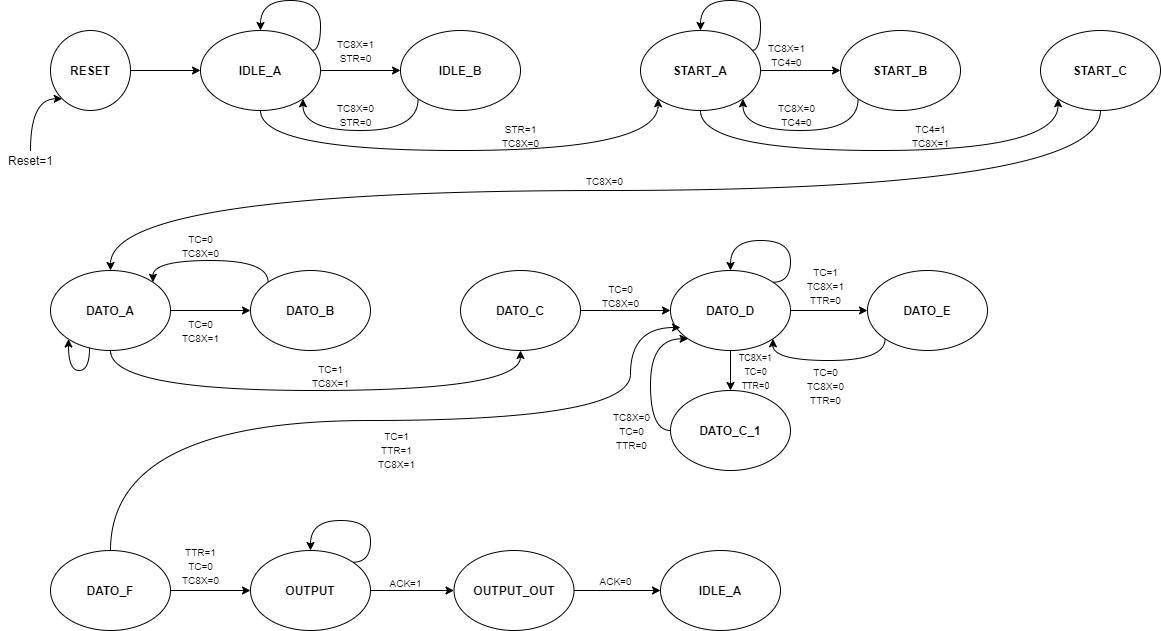
\includegraphics[scale=0.4]{PalleogrammaRXV2 (2).png}
    \caption{Palleogramma Rx}
    \label{fig:Pal-rx}
\end{figure}\\
In tale diagramma di stato, com'è stato fatto anche nella sezione precedente per il trasmettitore, per aiutare la comprensione dello schema ed evitare di intaccare la chiarezza, non sono state incluse tutte le connessioni da ogni stato a quello di "RESET" con la condizione RST=1.\\Quindi partendo dallo stato di "IDLE\_A", il sistema rimane lì finché non riceve i segnali che lo conducono in due possibili stati:
\begin{itemize}
    \item se TC8X=1 e STR=0, ovvero ancora non è avvenuta la transizione da IDLE a START, ma il contatore 8X ha terminato di contare, il sistema salta nello stato "IDLE\_B";
    \item se TC8X=0 e STR=1, ovvero se il contatore 8X non ha ancora terminato di contare, ma è avvenuta la start transition, allora il sistema salta nello stato "START\_A".
\end{itemize}
Successivamente in "IDLE\_B", al colpo di clock dopo, è presente la condizione TC8X=0 e STR=0, che permette di tornare in "IDLE\_A". Questo loop concede alla CU di inviare i comandi necessari al sovracampionamento.\\ Per quanto riguarda invece il caso in cui il sistema si trovi in "START\_A", si presenta nuovamente il caso con più strade ovvero il sistema resta in quello stato finché non arrivano diverse condizioni che lo portano in due differenti stati:
\begin{itemize}
    \item se TC8X=1 e TC4=0, ovvero il contatore 8X ha terminato di contare, mentre il contatore, che conta i 4 shift dopo il rilevamento della transizione, non ha ancora terminato di contare, allora il sistema salta nello stato "START\_B" e fa tutto ciò che deve fare per eseguire lo shift nello shift register;
    \item se TC8X=1 e TC4=1, cioè entrambi i contatori hanno terminato di contare, il sistema salta nello stato "START\_C".
\end{itemize}
In seguito a ciò, se il sistema è nello stato "START\_B", allora al colpo di clock successivo soddisferà le condizioni TC8X=0 e TC4=0, che lo riporteranno in "START\_A"; mentre se si trova nello stato "START\_C", al colpo di clock dopo, per TC8X=0, salterà in "DATO\_A", ovvero lo stato che indica l'inizio della ricezione del dato trasmesso.\\Una volta che il sistema è in questo stato, ha diverse possibilità a seconda delle condizioni che vengono soddisfatte, quindi questo resterà nello stato corrente fino a quando non avverrà che:
\begin{itemize}
    \item TC8X=1 e TC=0, ovvero il contatore 8X ha terminato di contare, mentre il contatore, che conta 2603 colpi di clock, non ha ancora terminato di contare, allora il sistema salta nello stato "DATO\_B";
    \item TC8X=1 e TC=1, cioè entrambi i contatori hanno terminato di contare, il sistema salta nello stato "DATO\_C".
\end{itemize}
Al colpo di clock successivo, per entrambi tali stati viene soddisfatta la condizione TC8X=0 e TC=0, che nel caso "DATO\_B", riporterà il sistema nello stato "DATO\_A", mentre nel caso "DATO\_C" lo porta nello stato "DATO\_D".\\Una volta in questo stato, il sistema si trova nuovamente a restare nello stato attuale oppure:
\begin{itemize}
    \item se TC8X=1, TC=1 e TTR=0, ovvero il contatore 8X ed il contatore 1 hanno terminato di contare, mentre il contatore 2, che conta i bit della word ricevuti, non ha ancora terminato di contare, allora il sistema salta nello stato "DATO\_E", questo loop permette di sovracampionare il dato in ricezione e di shiftare il bit ricevuto nel secondo shift register;
    \item se TC8X=1, TC=0 e TTR=0, cioè solo il contatore 8X ha terminato di contare, il sistema salta nello stato "DATO\_C\_1", questo loop è necessario in quanto solamente in istanti temporali particolari un bit della word è acquisito, però ogni volta che il contatore 8x finisce di contare si opera uno shift del sovracampionatore;
    \item se TC8X=1, TC=1 e TTR=1, indica che tutti e tre i contatori hanno terminato di contare e che la ricezione è entrata nella fase finale, il sistema si sposta in "DATO\_F".
\end{itemize}
A questo punto se il sistema si trova in "DATO\_E" oppure in "DATO\_C\_1", vengono soddisfatte le condizioni TC8X=0, TC=0 e TTR=0, che lo riportano in "DATO\_D". Se invece si trova in "DATO\_F", per TC8X=0, TC=0 e TTR=1 salta nello stato "OUTPUT", in cui nel secondo shift register entra l'ottavo e quindi ultimo dato trasmesso della word ed in cui si attiva OE2, ovvero l'abilitazione dell'uscita del dato interno al secondo shift register, dato che ora contiene l'intera word ricevuta dal trasmettitore.\\Successivamente con la condizione ACK=1, che è inviata dal sistema utilizzatore ed indica che questo ha ricevuto la word, in sistema salta in "OUTPUT\_OUT" e al colpo di clock successivo salta nuovamente nello stato iniziale "IDLE\_A" in base alla condizione ACK=0.
\subsection{Simulazione Modelsim}
Al fine di testare il corretto funzionamento del ricevitore è stato deciso di far ciò sfruttando l'intera UART, il dato ricevuto è stato fornito dal trasmettitore della stessa. Tale test è descritto nella sezione relativa alla UART.
\newpage
\section{Uart}
%subsection{QUESTO C'è ANCHE SOTTO, SCEGLIETE QUALE VI PIACE DI PIU'}
%.\\Si è proceduto scegliendo su Quartus 18.1 la FPGA ALTERA Cyclone V "5CSEMA5F31C6N" fornita dal laboratorio.\\L'obiettivo finale è stato quello di creare un collegamento tra i nostri segnali e i pin della FPGA, ciò è stato possibile attraverso il Pin Assignment.\\I segnali sono stati mandati su KEY, SWITCH e LED per verificare la trasmissione di dati con l'illuminazione dei LED. Il Data\_out, importato attraverso gli SWITCH segue tutte le volte un dato iter: passa dal trasmettitore al ricevitore e successivamente va ad accendere il LED per attestare l'avvenuta ricezione del dato.\\ Il Data Valid, l'Acknoledge, Rx\_ack e il Reset sono impostati attraverso le Keys,rispettivamente \textbf{Key(1)},\textbf{Key(2)} e \textbf{Key(0)}. Associamo a LEDR da 0 a 7 il \textbf{Data\_in}, mentre i \textbf{Data\_out} sono collegati agli Switch.\\Il \textbf{Tx\_ready} è invece legato a LEDR(9), mentre \textbf{Rx\_ready} è collegato a LEDR(8).\\Avendo una scheda (DE1) con clock disponibile solo a 50 MHz, si è dovuto creare un blocco utilizzato come divisore di frequenza, che effettui un dimezzamento.\\Tale blocco è stato realizzato utilizzando un PLL di Intel.

Il progetto finale consiste nel design di una UART completa, riportata precedentemente in Figura \ref{fig:UART}, e per tale motivo è stata progettata una top level entity, che racchiudesse sia il ricevitore che il trasmettitore.\\
\subsection{Simulazione su Modelsim}
Le verifiche preliminari del sistema sono state effettuate nell'ambiente Modelsim, simulando via software tutti i segnali necessari all'invio e alla ricezione di un dato, per fare ciò è stato collegato il trasmettitore insieme al ricevitore. I risultati della simulazione sono visibili in Figura \ref{fig:sim_rx}.
\begin{figure}[h]
    \centering
    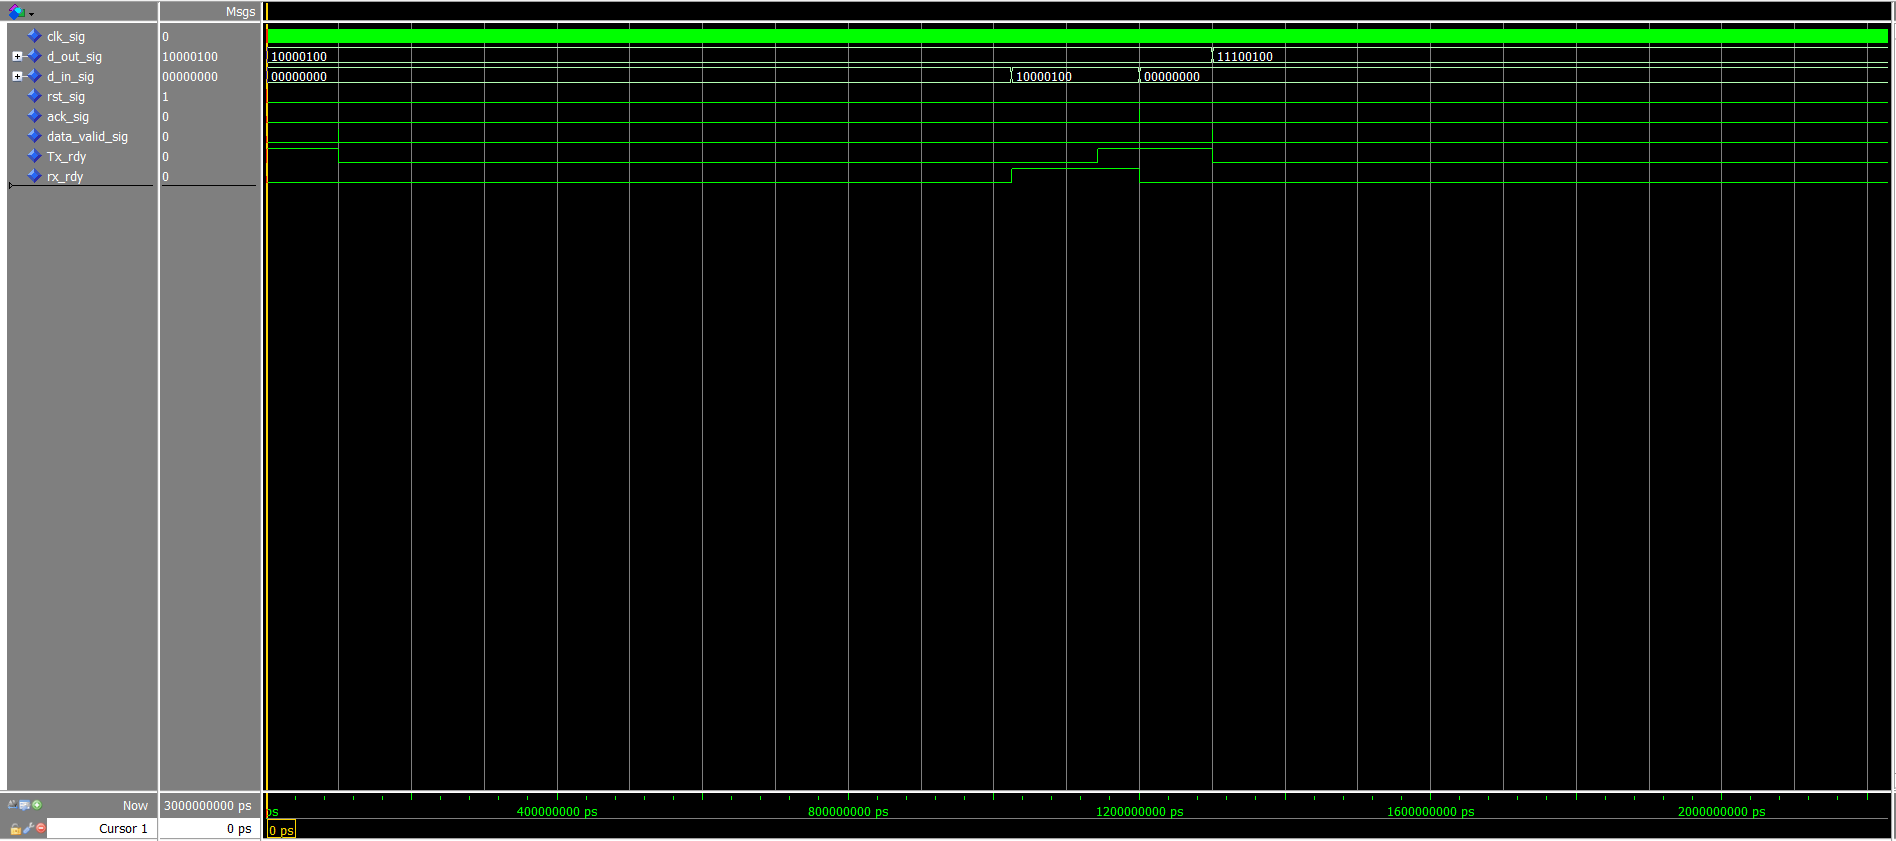
\includegraphics[scale=0.4]{test_RX.PNG}
    \caption{Simulazione di una ricezione}
    \label{fig:sim_rx}
\end{figure}\\
Dalla simulazione è possibile notare nettamente che il dato trasmesso viene ricevuto dopo un certo lasso di tempo (dettato dal tempo di bit), insieme alla ricezione e alla presentazione del dato viene alzata anche la linea "RX \textunderscore RDY". Il ricevitore mantiene il dato ricevuto finché non viene assegnato  l' "ACK", in seguito il bus è posto a zero in attesa di una nuova ricezione. Come si può notare anche dalla simulazione Modelsim, il dato trasmesso è lo stesso ricevuto.
\subsection{Test su Board DE1}
La verifica finale del sistema è stata fatta progettando un ulteriore top-level per sfruttare gli switch, i led e i button della board, questo è stato fatto utilizzando il Pin Assignment di Quartus, i test sono stati condotti sulla  FPGA ALTERA Cyclone V "5CSEMA5F31C6N" fornita dal laboratorio. E' stato deciso di mostrare il dato ricevuto sui led, il dato è stato inserito tramite gli switch così da cambiare il contenuto della word ad ogni trasmissione, mentre il reset è stato collegato all'interruttore a bottone. Dato che vi era la necessità di verificare il risultato tramite i led, è stato sfruttato un contatore con un delay adeguato per generare il "DATA \textunderscore VALID". Tale contatore è fornito di un counter enable collegato ad uno switch. Quindi con tale sistema è stato possibile avere controllo delle trasmissioni con un timing adeguato a verificare il corretto funzionamento. Il segnale di Acknowledgement è stato fornito tramite uno switch.\\Inoltre tale sistema lavora a 25 MHz, ma la scheda DE1 forniva solo un clock a 50 MHz, quindi è stato reso necessario l'utilizzo di un PLL, implementato utilizzando le librerie Intel disponibili su Quartus.
\newline
Le periferiche utilizzate sono:
\begin{itemize}
    \item KEY(0): Reset
    \item KEY(1): ACK
    \item LEDR(9): TX \textunderscore RDY
    \item LEDR(8): RX \textunderscore RDY
    \item SW(7 downto 0): D \textunderscore OUT
    \item SW(8): Enable (contatore esterno)
    \item LEDR(7 downto 0): D \textunderscore IN
\end{itemize}
Lo schema a blocchi del test hardware è riportato in figura \ref{fig:Fpgatest}.
\begin{figure}[!h]
    \centering
    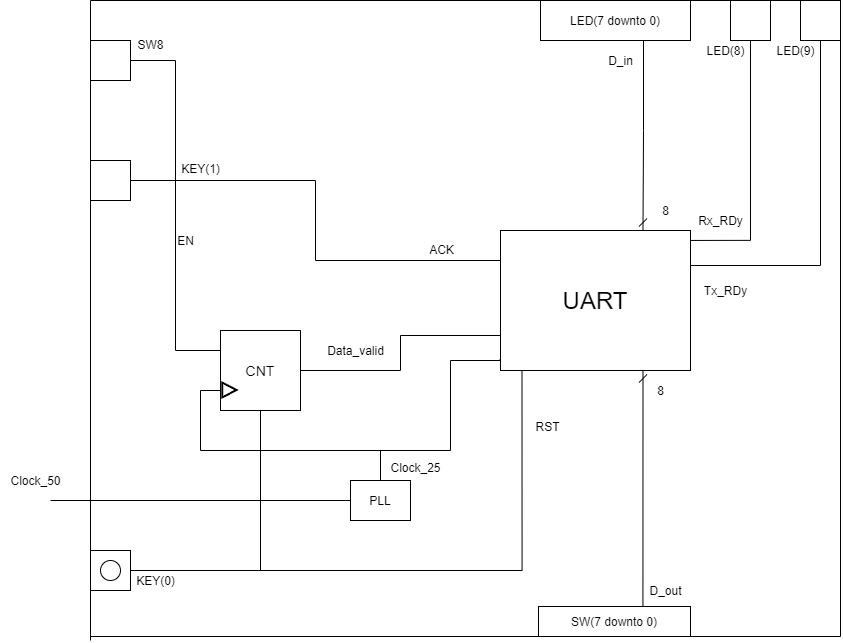
\includegraphics[scale=0.5]{FPGAtest.png}
    \caption{FPGA test}
    \label{fig:Fpgatest}
\end{figure}
\\Di seguito nelle Figure \ref{fig:test_1}, \ref{fig:test_2}, \ref{fig:test_3} sono riportati i vari test effettuati in laboratorio con la board DE1.
\begin{figure}[h]
    \centering
    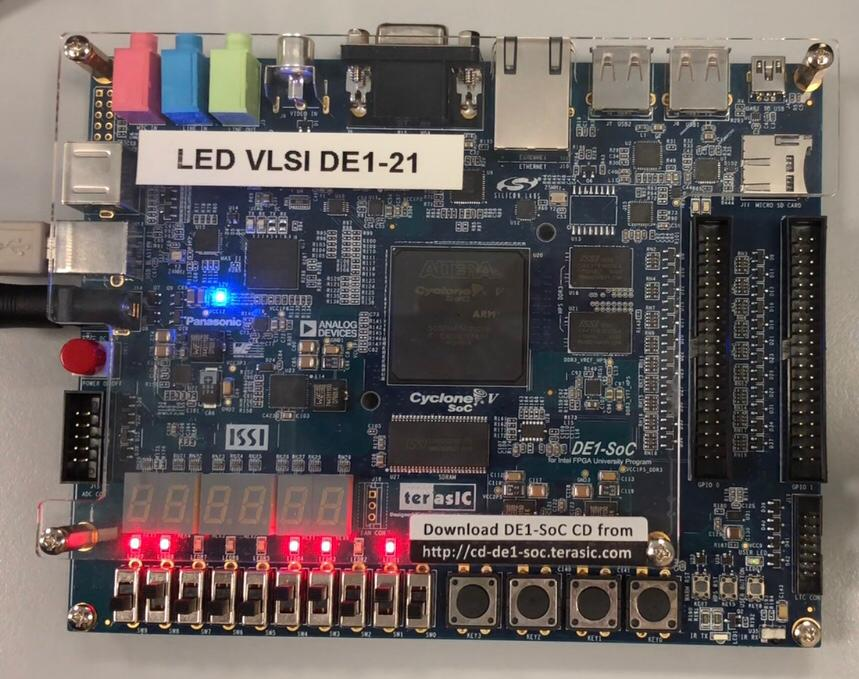
\includegraphics[scale=0.30]{WhatsApp Image 2020-03-12 at 18.31.33.jpeg}
    \caption{Test con dato trasmesso D \textunderscore OUT=00011010}
    \label{fig:test_1}
\end{figure}
\newpage
\begin{figure}[h]
    \centering
    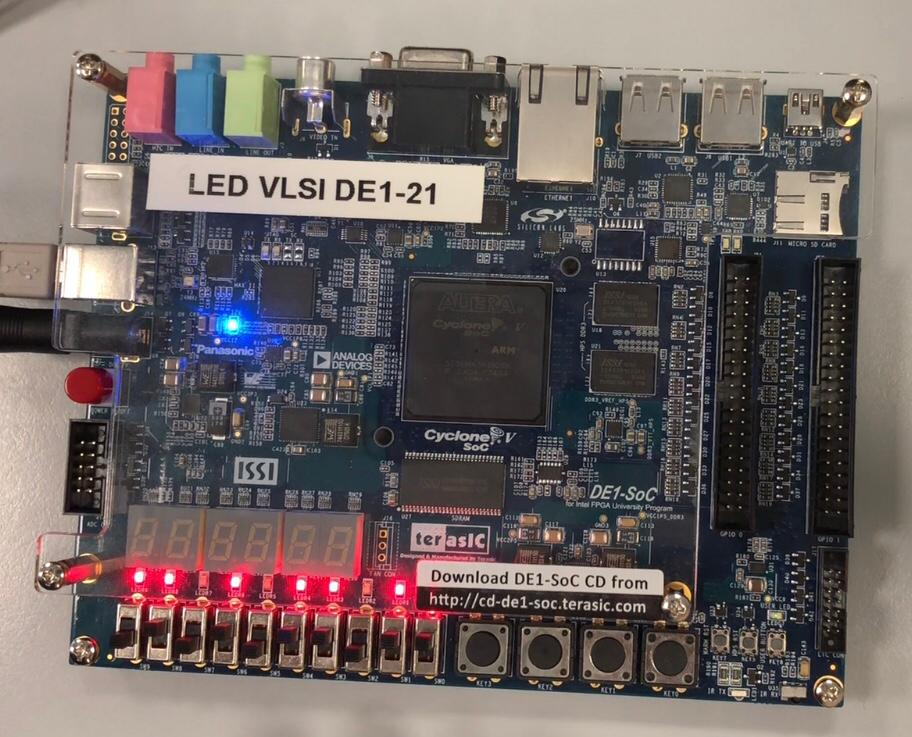
\includegraphics[scale=0.30]{WhatsApp Image 2020-03-12 at 18.31.44.jpeg}
    \caption{Test con dato trasmesso D \textunderscore OUT=01011011}
    \label{fig:test_2}
\end{figure}
\begin{figure}[h]
    \centering
    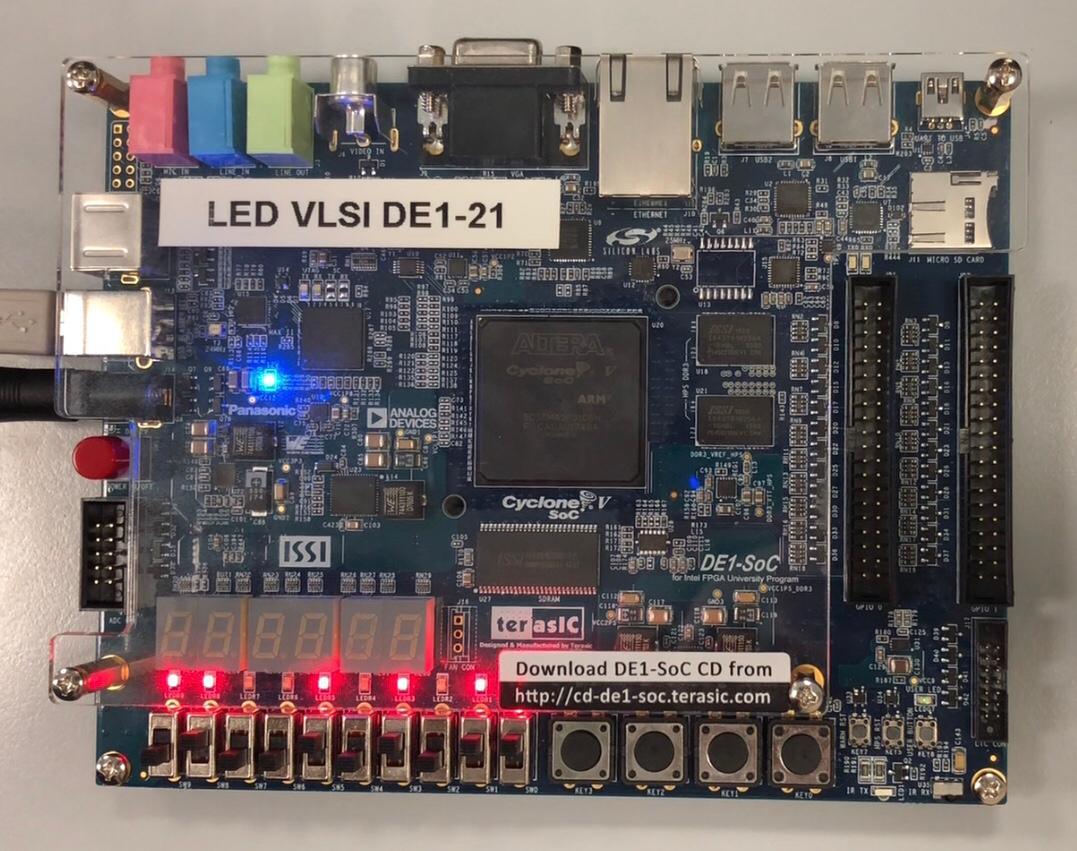
\includegraphics[scale=0.25]{WhatsApp Image 2020-03-12 at 18.31.54.jpeg}
    \caption{Test con dato trasmesso D \textunderscore OUT=00101011}
    \label{fig:test_3}
\end{figure}
La validità dei test può essere verificata tramite i valori assunti dagli switch e i led accesi.\\Tutti i test eseguiti hanno dato esito positivo.
\begin{sidewaysfigure}
\centering
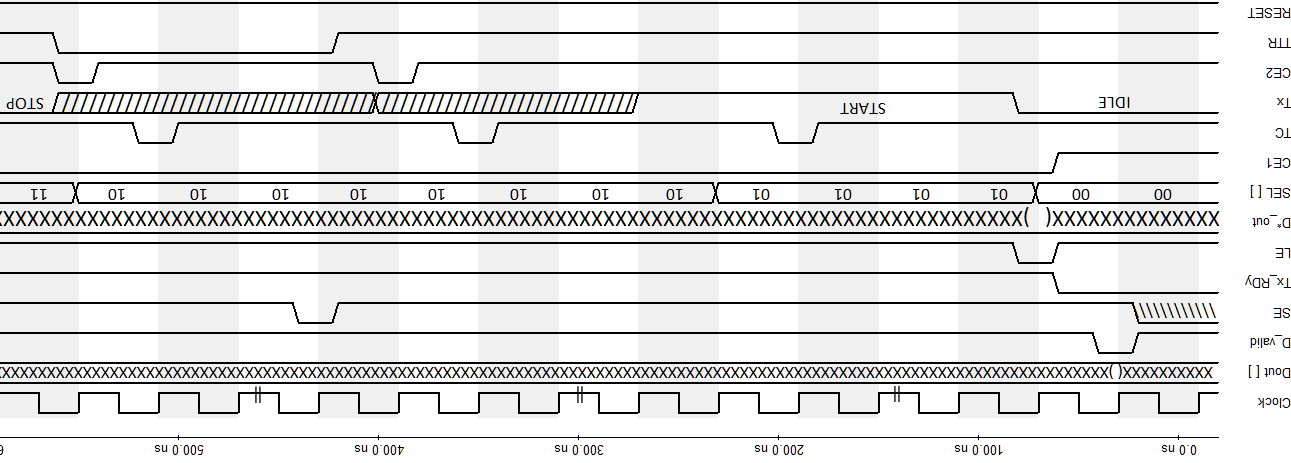
\includegraphics[scale=0.7]{timingtxV6_1.png} 
\caption{Timing trasmettitore}
\label{TX Timing}
\end{sidewaysfigure}
\begin{sidewaysfigure}
\centering
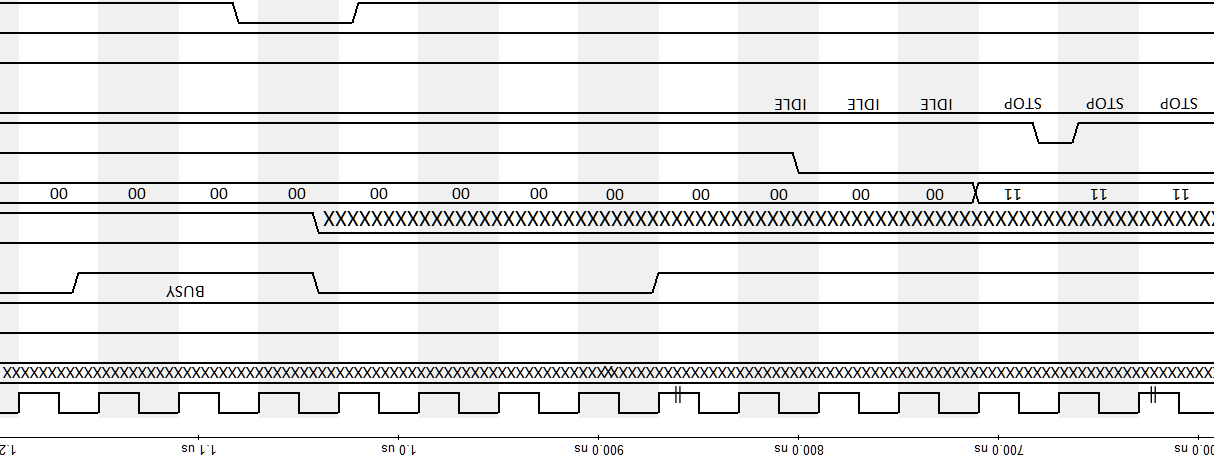
\includegraphics[scale=0.7]{timingtxV5_2.png} 
\end{sidewaysfigure}

\begin{sidewaysfigure}
\centering
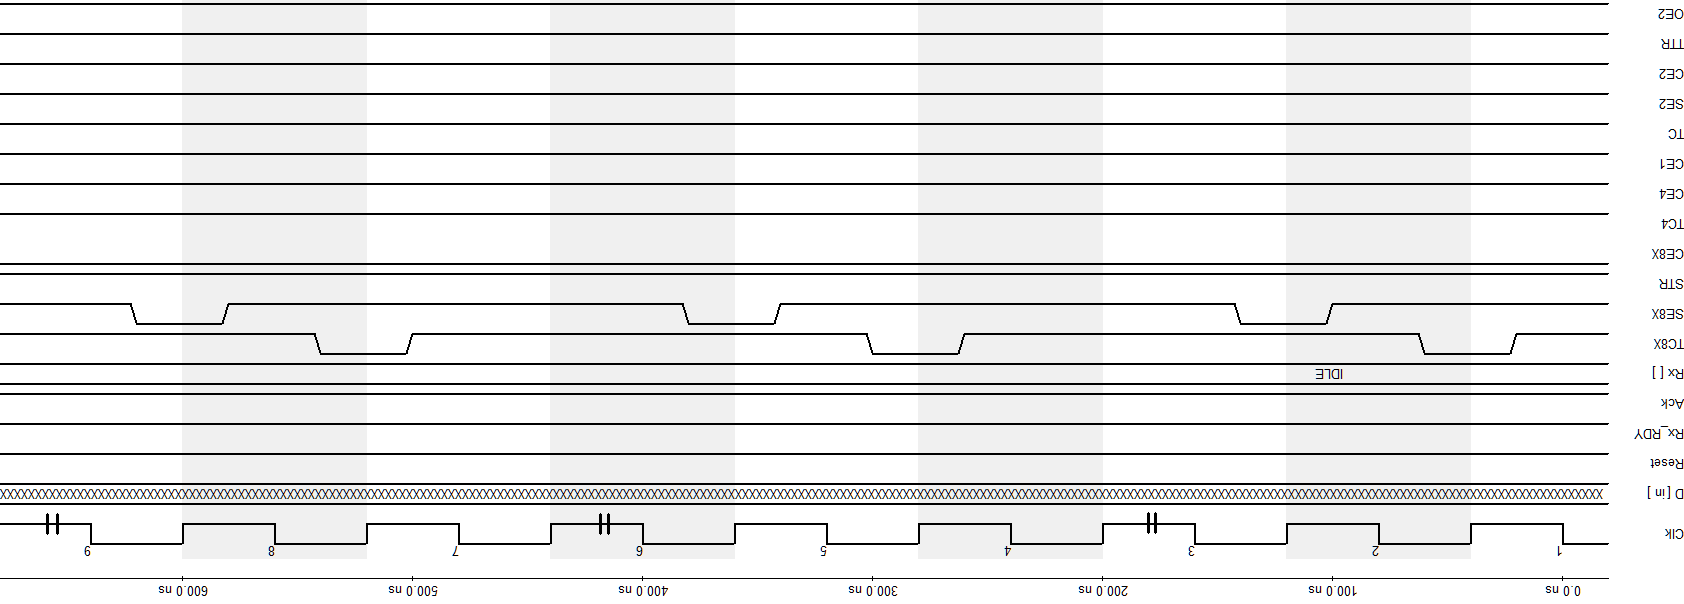
\includegraphics[scale=0.6]{RX_timing_pt1.png} 
\caption{Timing Ricevitore}
\label{RX Timing}
\end{sidewaysfigure}
\begin{sidewaysfigure}
\centering
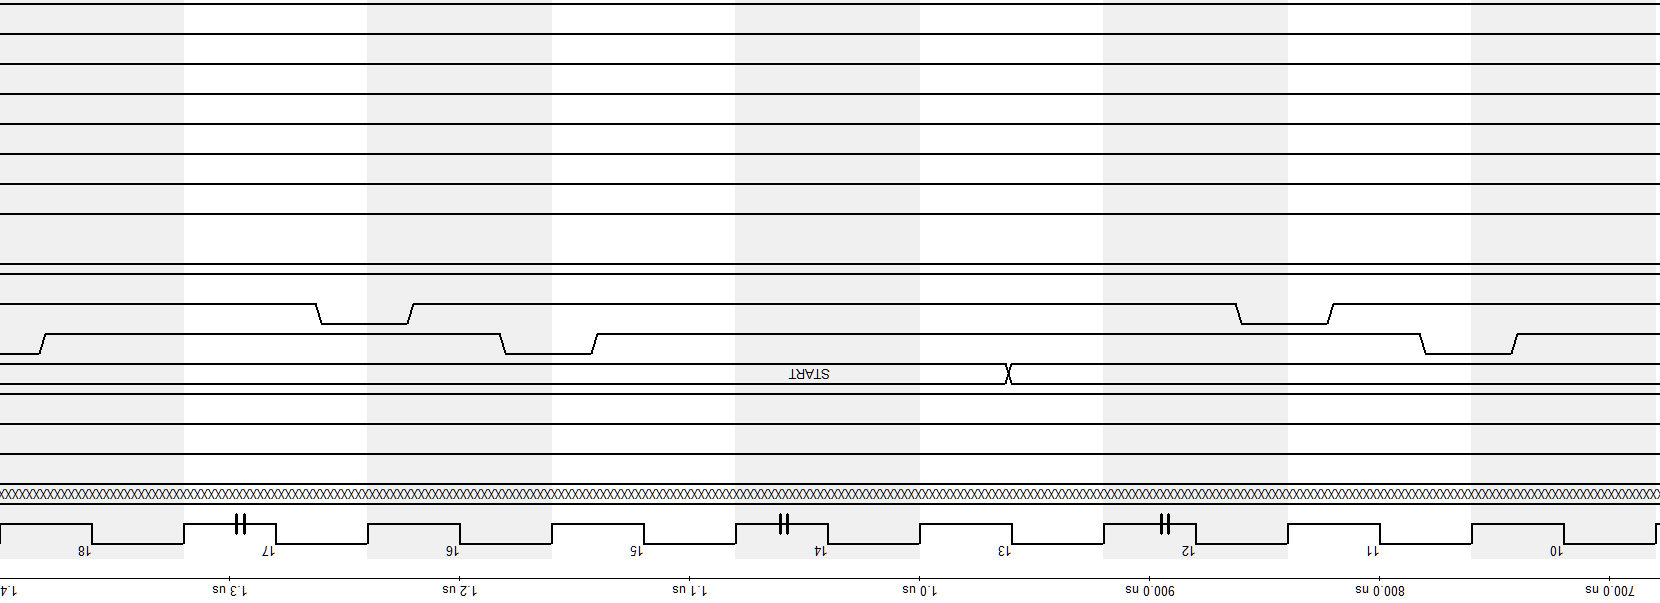
\includegraphics[scale=0.6]{RX_timing_pt2.png} 
\end{sidewaysfigure}
\begin{sidewaysfigure}
\centering
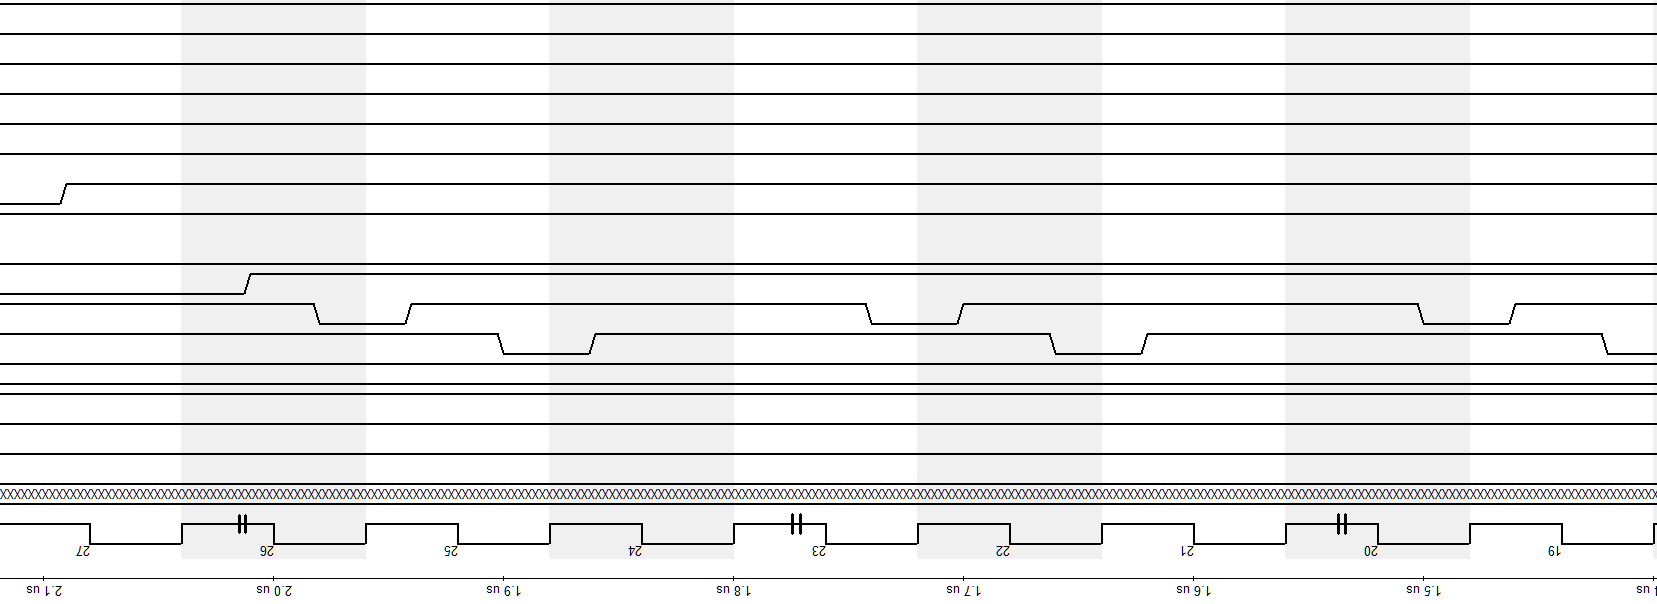
\includegraphics[scale=0.6]{RX_timing_pt3.png} 
\end{sidewaysfigure}
\begin{sidewaysfigure}
\centering
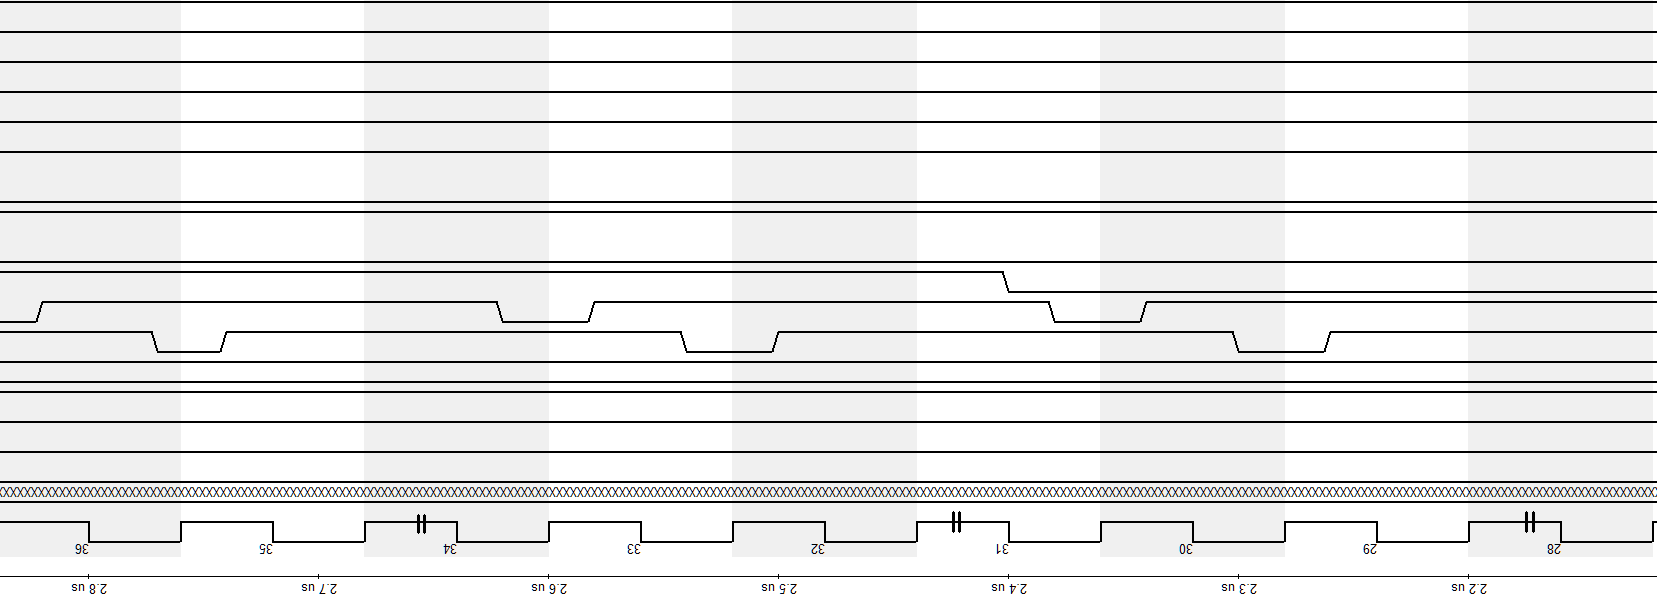
\includegraphics[scale=0.6]{RX_timing_pt4.png} 
\end{sidewaysfigure}
\begin{sidewaysfigure}
\centering
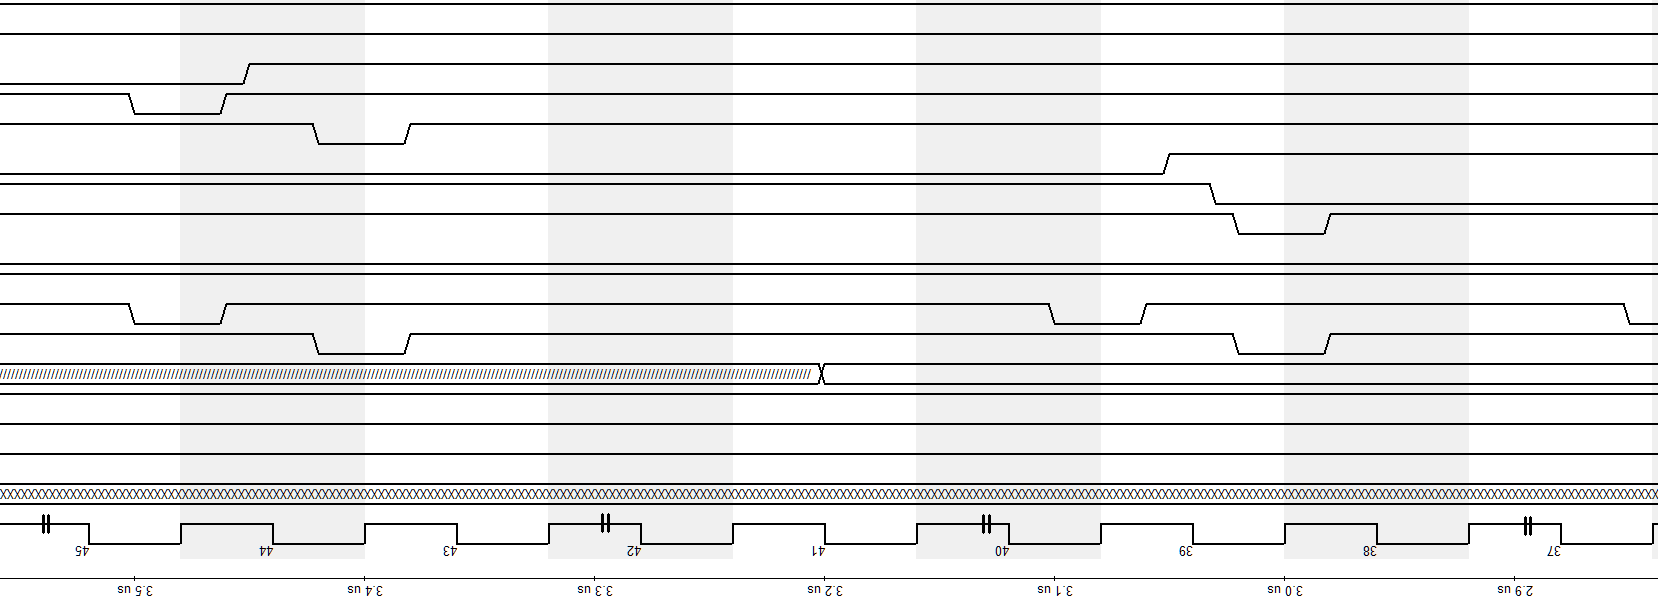
\includegraphics[scale=0.6]{RX_timing_pt5.png} 
\end{sidewaysfigure}
\begin{sidewaysfigure}
\centering
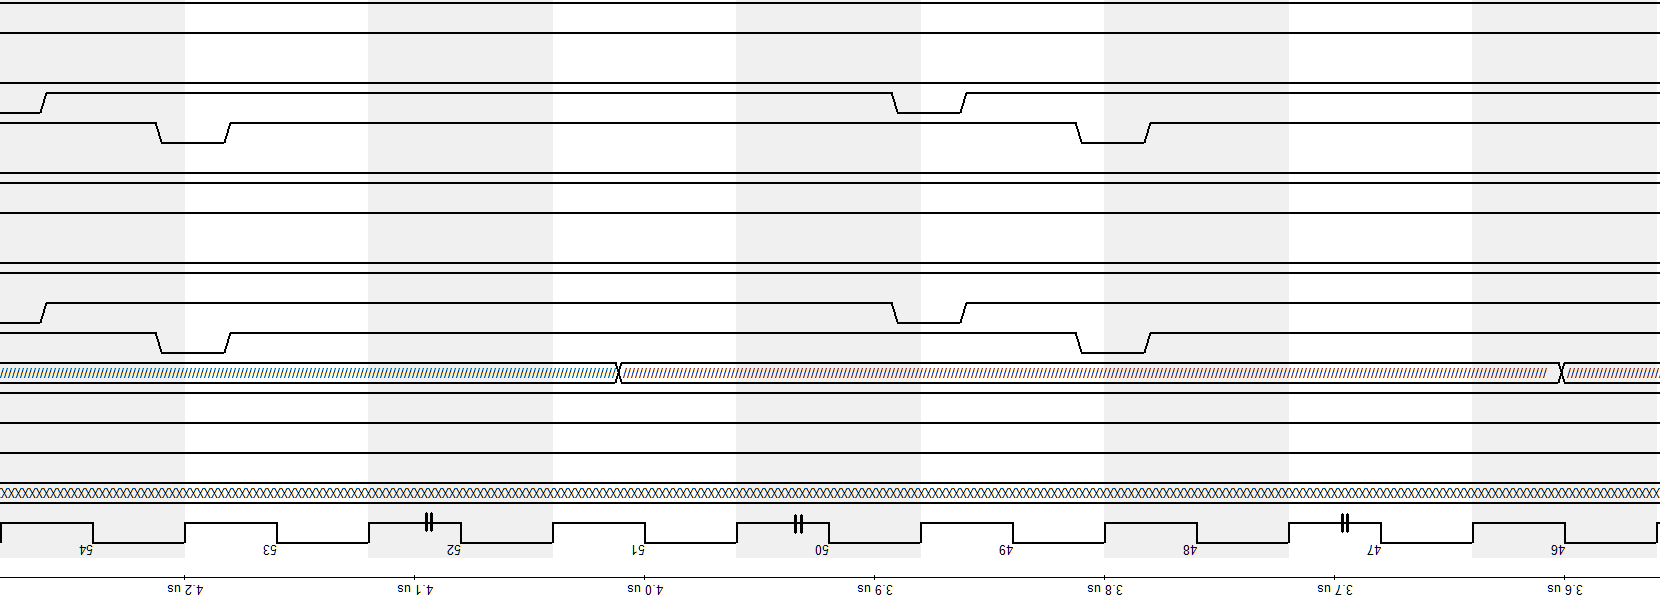
\includegraphics[scale=0.6]{RX_timing_pt6.png} 
\end{sidewaysfigure}
\begin{sidewaysfigure}
\centering
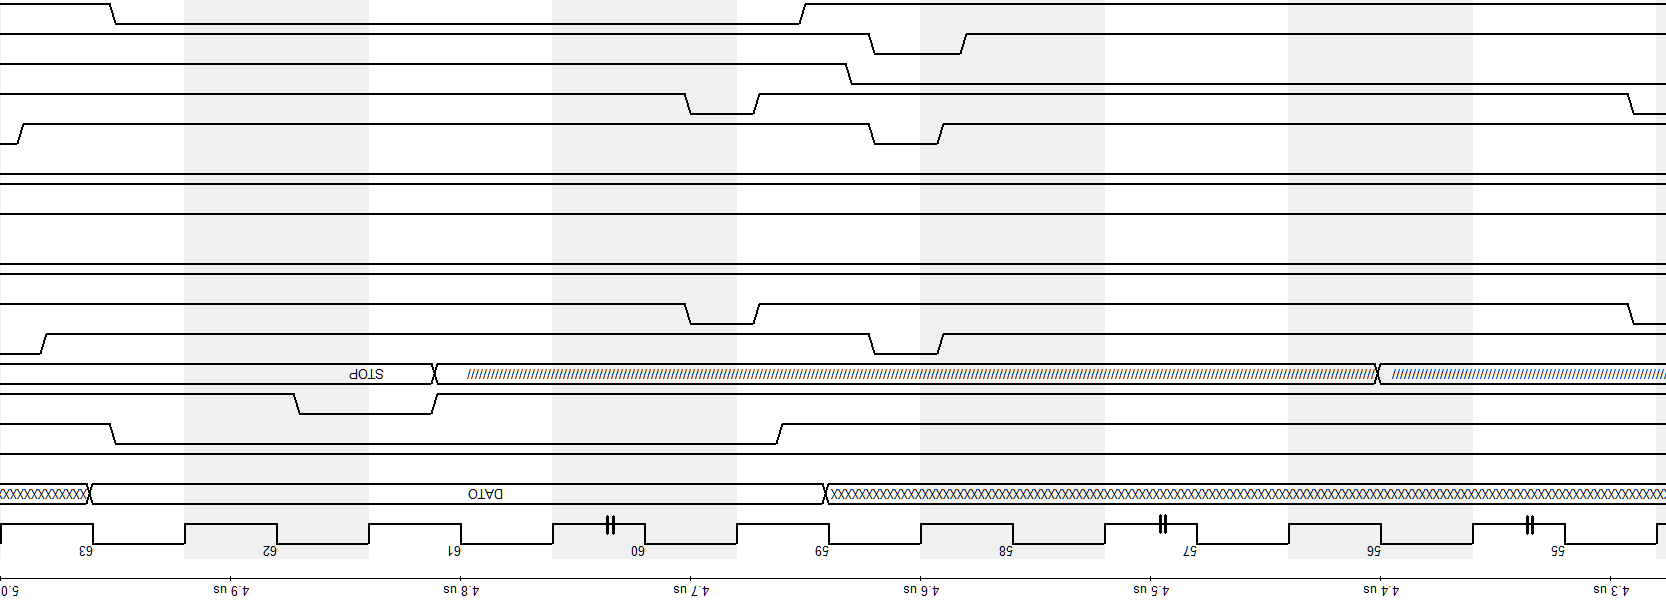
\includegraphics[scale=0.6]{RX_timing_pt7.png} 
\end{sidewaysfigure}
\begin{sidewaysfigure}
\centering
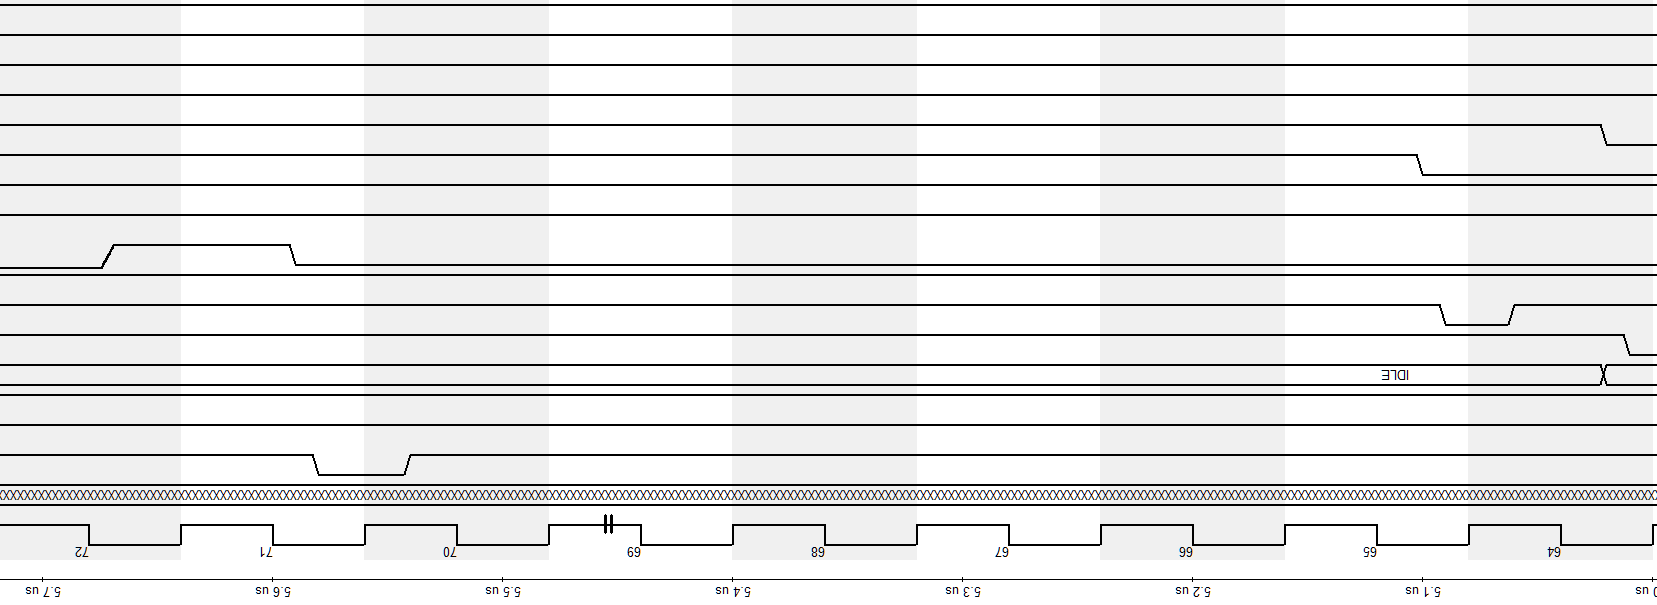
\includegraphics[scale=0.6]{RX_timing_pt8V2.png} 
\end{sidewaysfigure}
%\begin{sidewaysfigure}[t]
%\centering
%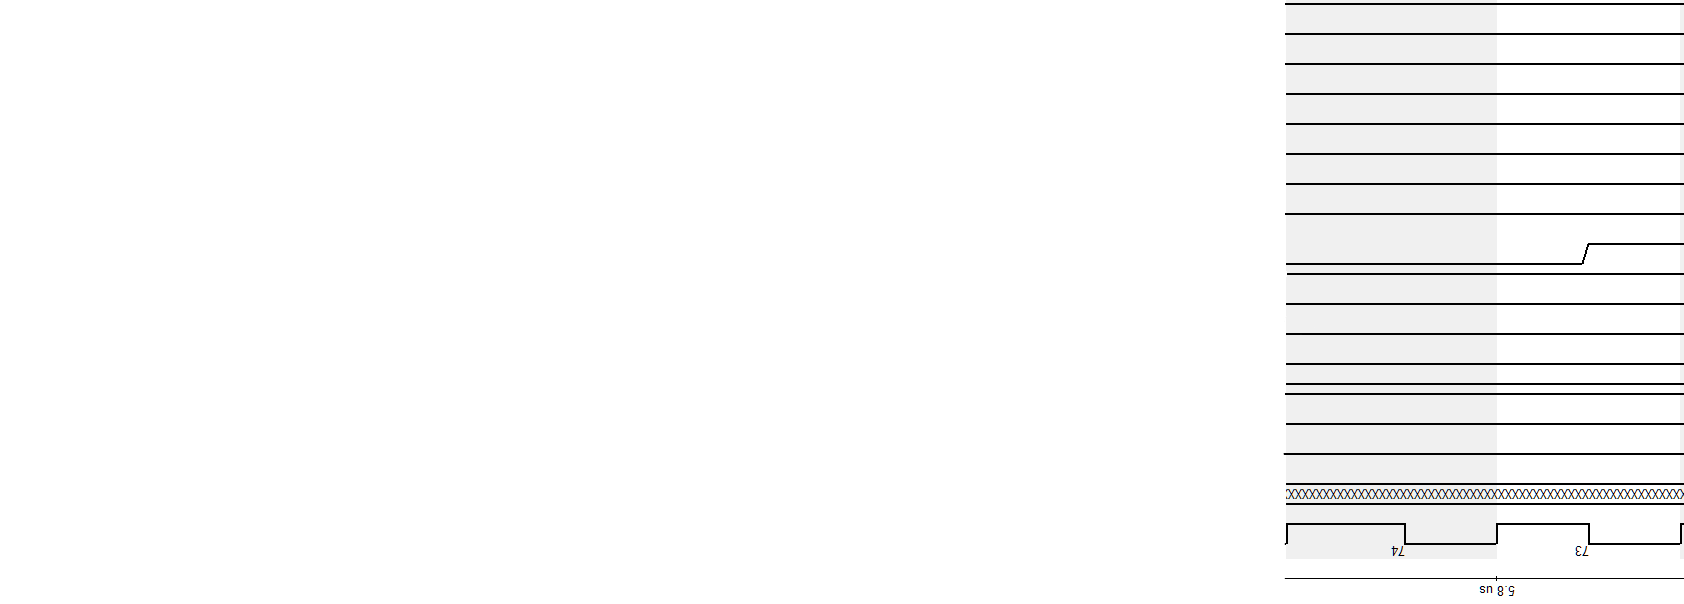
\includegraphics[scale=0.6]{RX_timing_pt10.png} 
%\end{sidewaysfigure}
\end{document} 